\section{Background}
\label{sec:Background}

\subsection{DREMS Infrastructure}
%\subsubsection{The Component Model}
%\label{sec:The_Component_Model}

%The DREMS platform is characterized by a hierarchical scheduling scheme. The higher, component-level scheduler schedules component operations for execution, enabling interactions between application components. The lower, operating system scheduler enforces a temporal partitioning scheme and schedules the component threads. Components are grouped into unique, identifiable processes called actors. These actors are assigned to temporal partitions and run only when the associated temporal partition is active. This partitioned scheduling provides a guaranteed slice of the CPU to all the actors and enables isolation between multiple applications running on the same computing node.

\subsubsection{DREMS Components}
\label{sec:drems_component}
%\vspace{0.1in}
Design and implementation of component-based software applications rests on the principle of assembly: \textit{Complex systems can be built by composing re-useable interacting components}. Components contain functional, business logic code that implements operations on state variables. Ports facilitate interactions between communicating components. A component-level message queue, with associated infrastructure code, controls the scheduling of operations on the individual components. Figure \ref{fig:drems_component} shows a basic DREMS component.  

%\vspace{-0.07in}
\begin{figure}[ht]
\centering
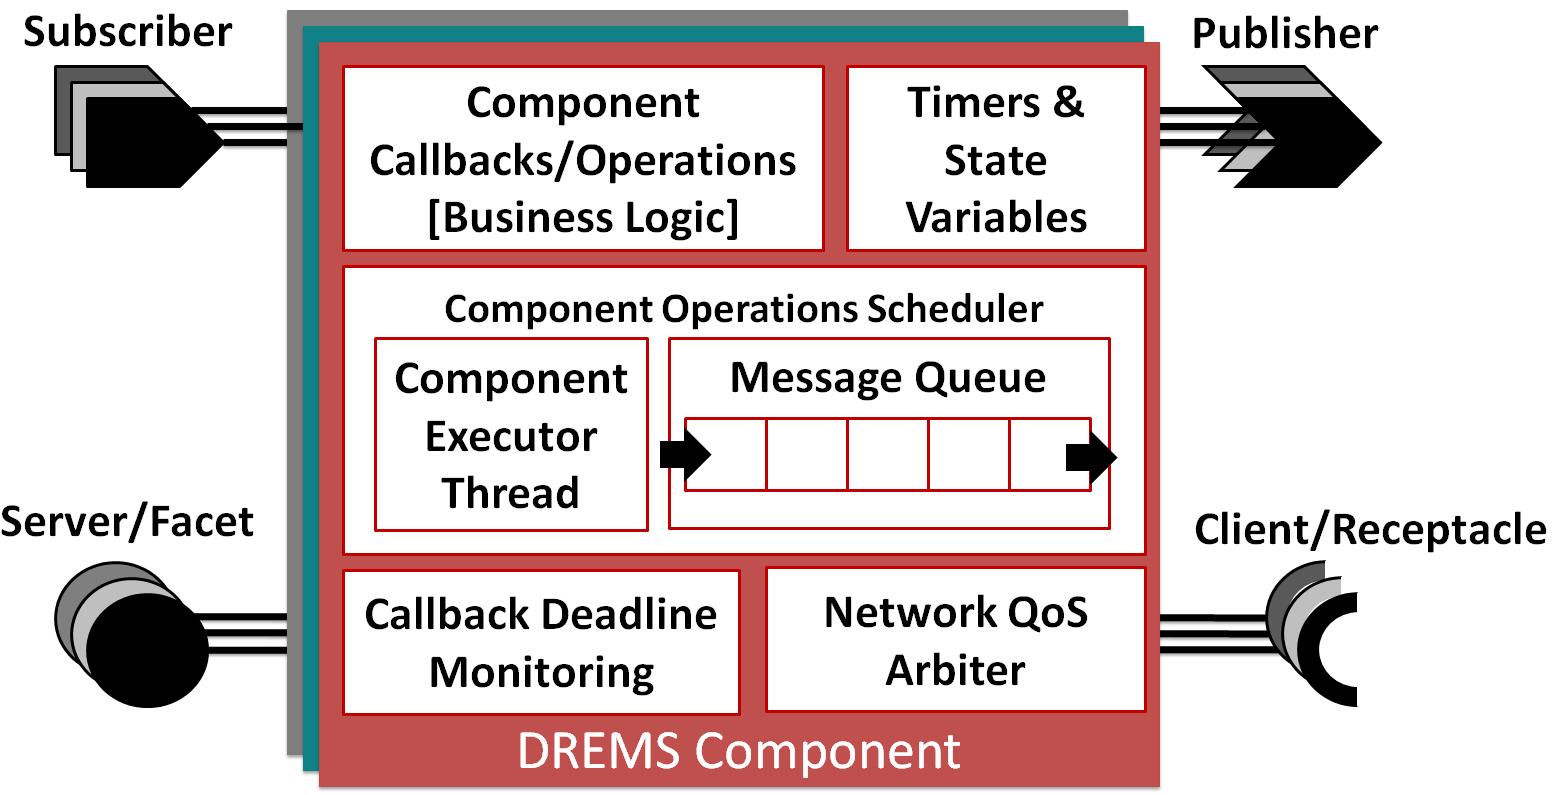
\includegraphics[width=0.35\textwidth]{drems_component}
\caption{DREMS Component}
\label{fig:drems_component}
\vspace{-0.2in}
\end{figure}
\vspace{0.1in}

Each DREMS component supports four basic types of ports for interaction with other collaborating components: Facets, Receptacles, Publishers and Subscribers. A component's {\bf facet} is a unique interface that it exposes to its clients. This interface can be invoked either synchronously via remote method invocation (RMI) or asynchronously via asynchronous method invocation (AMI). A component's {\bf receptacle} specifies an interface required by the component in order to function correctly. Using its receptacle, a component can establish connections and invoke operations on other components using either RMI or AMI. A {\bf publisher} port is a single point of data emission. This port emits data produced by a component operation. A {\bf subscriber} port is a single point of data consumption, feeding received data to the associated component. Communication between publishers and subscribers is contingent on the compatibility of their associated topics. Publishers and Subscribers enable the OMG DDS anonymous publish/subscribe style of messaging. More details on this component model can be found in ~\cite{ISIS_F6_ISORC:13}.

%Additionally, this component model also supports sporadic and periodic timers that can be used to initiate component operations. 


\subsubsection{Component Operations}
\label{sec:component_operations}
An operation is an abstraction for the different tasks undertaken by a component. These tasks are implemented by the component's executor code written by the developer. In order to service interactions with the underlying framework and with other components, every component is associated with a message queue. This queue holds instances of operations ('messages') that are ready for execution and need to be serviced by the component. These operations service either interaction requests (seen on communication ports) or service requests (from the underlying framework). An example for the latter is the use of component timers that can periodically (or sporadically) activate an operation. 

Figure \ref{fig:component_operations} shows the basic structure of this model. Each operation is characterized by a priority and a deadline. Operation deadlines are quantified in absolute time measured starting from when the operation is enqueued onto the component message queue. %These operations are sorted and scheduled based on one of three scheduling schemes: Earliest Deadline First (EDF), First In First Out (FIFO), and Priority FIFO. 

\vspace{-0.12in}
\begin{figure}[ht]
\centering
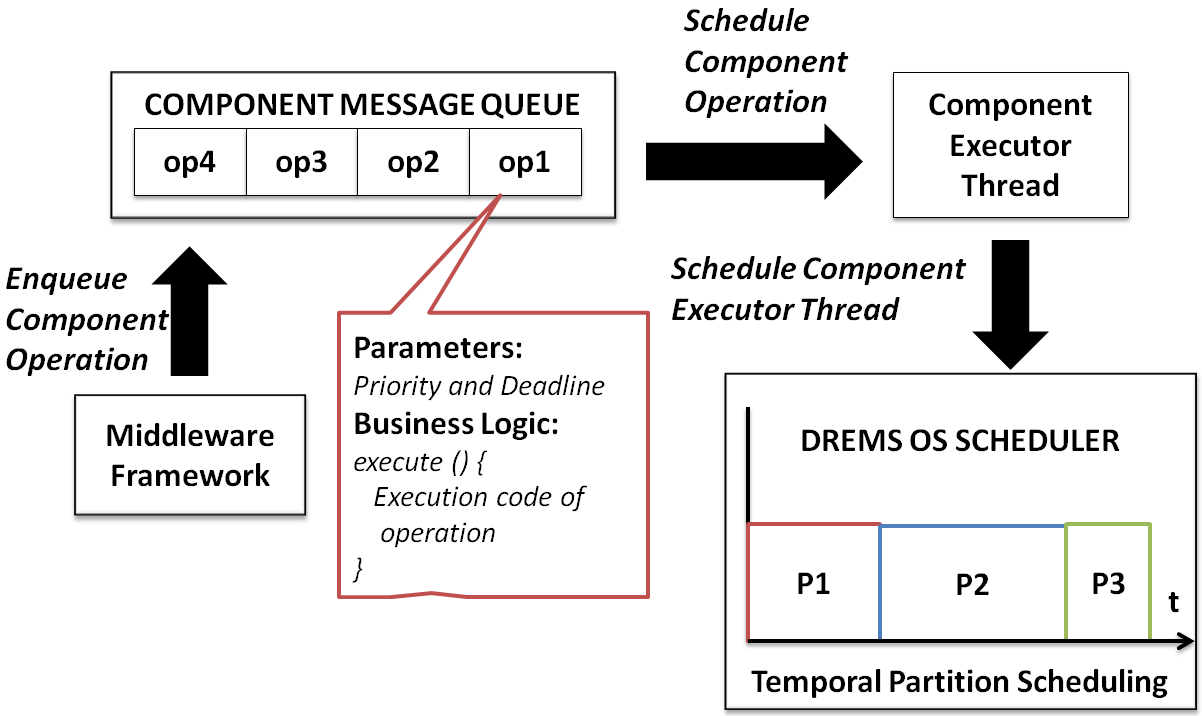
\includegraphics[width=0.4\textwidth]{component_operations}
\caption{Scheduling Component Operations}
\label{fig:component_operations}
\vspace{-0.18in}
\end{figure}
%\vspace{0.2in}

To facilitate component behavior that is free of deadlocks and race conditions, the component's execution is handled on a single thread. Operations in the message queue are therefore scheduled one at a time under a non-preemptive policy. A component dispatcher thread dequeues the next ready operation from the component message queue. This operation is scheduled for execution on a component executor thread. The operation is run to completion before another operation from the queue is serviced. This single-threaded execution helps avoid synchronization primitives such as internal state variables that lead to strenuous code development. Though components that share a processor still run concurrently, each component operation is executed on a single component-specific executor thread.

Figure \ref{fig:timing_diagram} shows a sample timing diagram of how a component operation is handled. At time 0, the component executor thread is running some previously ready component operation, \emph{op1}. At this point, consider that a new component operation \emph{op2} is enqueued onto the message queue and marked as ready. At time 10, assuming that no other component requires scheduling, the component dispatcher thread of this component dequeues the next ready operation for execution. Assuming the component executor thread is scheduled immediately by the underlying processor, this thread runs the ready operation by invoking its \emph{execute} function. This operation is run to completion at time 16. The total time taken for execution of this operation is measured from when the operation was enqueued, i.e. time 0. If the time taken for the operation exceeds its deadline, a fault manager is immediately notified. The duration of the component operation is further delayed by temporal partitioning enforced by the OS scheduler. This adds to the need for schedulability analysis, especially in case of safety and mission-critical applications.

\begin{figure}[ht]
\centering
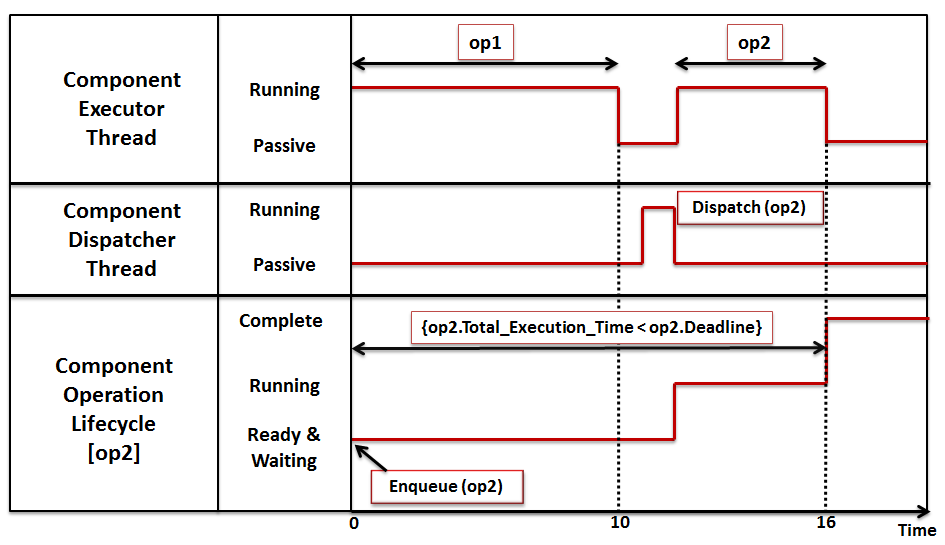
\includegraphics[width=0.50\textwidth]{cop_timing_diagram}
\caption{Component Operation Execution}
\label{fig:timing_diagram}
\vspace{-0.2in}
\end{figure}
\vspace{0.1in}
